\documentclass[final,hyperref={pdfpagelabels=false},xcolor=table]{beamer}
\mode<presentation>{
	\usetheme{ucb}
}
\usepackage[size=custom,width=101.6,height=76.2,scale=1.5]{beamerposter}
\usepackage{multicol}
\usepackage{graphicx}
\usepackage{textcomp}
\usepackage{pbox}
%\usepackage{booktabs}
%\usepackage{multirow}
%\usepackage{listings}
\usepackage{siunitx}
\usepackage{blindtext}

\definecolor{ucb-pacific}{HTML}{5B6770}

\newcommand{\uT}{{\textmu}T}
\setlength{\leftmargini}{4em}

\title{Hardware Acceleration of Key-Value Stores}
\author{Sagar Karandikar, Howard Mao, Albert Ou, Soumya Basu}
\advisor{Krste Asanovi\'{c}}
\institute[UC Berkeley]{\textsc{University of California, Berkeley}}
\date[2014-12-11]{CS262a, 11 December 2014}

\begin{document}
\begin{frame}
\vspace{-1.5em}
\begin{columns}[t]
	\begin{column}{0.3\linewidth}
	\begin{block}{Motivation}
We want to bypass the CPU entirely and be able to serve hot requests in
hardware. The software stack of the end host takes about 86-95 percent of the
total latency, so substantial speed gains can be made here.

\end{block}

\vspace{1ex}

\begin{block}{Related Work}
\end{block}

    \vspace{1ex}
    \begin{block}{Infrastructure}
\footnotesize

\begin{minipage}{0.4\linewidth}
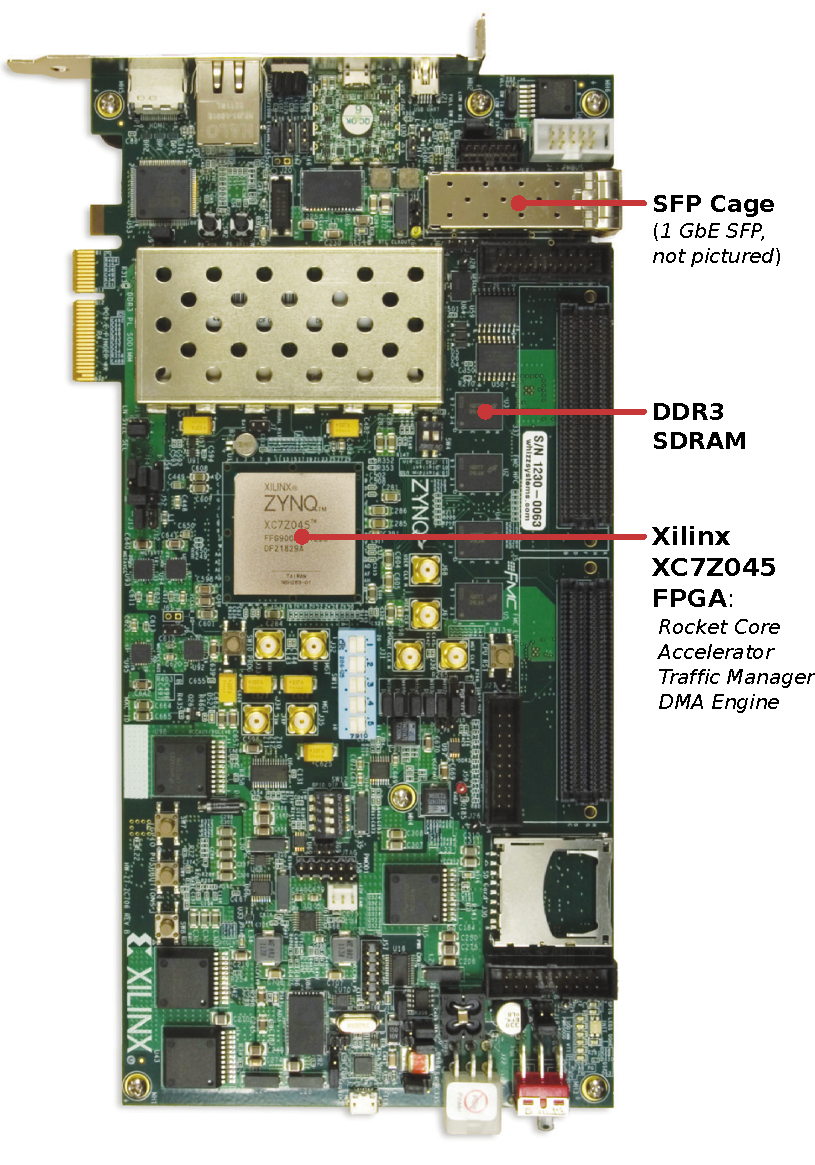
\includegraphics[width=\linewidth]{img/zc706.pdf}
\end{minipage}
\hfill
\begin{minipage}{0.55\linewidth}
\alert{Xilinx ZC706 Evaluation Platform}
\begin{itemize}
\item ZYNQ-7000 SoC
\item Brocade 1GbE Copper SFP Transceiver
	\begin{itemize}
	\footnotesize
        \item Xilinx Tri-Mode Ethernet MAC
        \item Xilinx 1000Base-X PCS/PMA
	\end{itemize}
\item 64-bit RISC-V Rocket Core (\SI{50}{\mega\hertz})
	\begin{itemize}
	\footnotesize
	\item Single-issue, in-order, 6-stage pipeline
	\item ASIC version most nearly comparable with ARM Cortex-A5
	\end{itemize}
\end{itemize}
\vspace{\baselineskip}
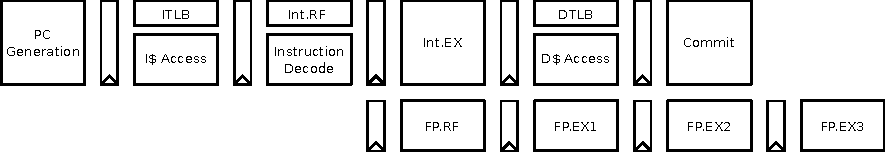
\includegraphics[width=\linewidth]{img/rocket-pipeline.pdf}
\end{minipage}

\hrule
\vspace{0.5\baselineskip}
\begin{itemize}
\item No pre-existing I/O peripherals for the Rocket chip
\item Built first RISC-V hardware device: register-mapped NIC
	\begin{itemize}
	\footnotesize
	\item First \texttt{telnet/ssh} into a physical RISC-V machine
	\end{itemize}
\item Evolved to DMA-based NIC for performance
\end{itemize}
 
\end{block}

	\end{column}

	\begin{column}{0.3\linewidth}
    \begin{block}{System Architecture}
\begin{multicols}{2}
\centering
\alert{Baseline} \\[0.5\baselineskip]
\includegraphics[scale=1.45]{img/system-base.pdf}

\columnbreak

\centering
\alert{Enhanced} \\[0.5\baselineskip]
\includegraphics[scale=1.45]{img/system-kvstore.pdf}
\end{multicols}
\end{block}

\vspace{1ex}

\begin{block}{Accelerator}
\footnotesize

\begin{multicols}{2}
\begin{center}
    \alert{Accelerator} \\[0.5\baselineskip]
    \includegraphics[width=\linewidth]{img/kvstore.pdf}
\end{center}

\columnbreak

\begin{center}
    \alert{Traffic Manager} \\[0.5\baselineskip]
    \includegraphics[width=\linewidth]{img/frontend.pdf}
\end{center}

\end{multicols}

\begin{itemize}
    \item The accelerator accepts a key and computes primary and secondary
        hash values, which it uses to retrieve the value from its local
        block RAM.
    \item The traffic manager, interposed between the NIC and the DMA
        engine, implements the specialized Memcached logic.
	For intercepted Memcached GET requests, it queries the
	accelerator and constructs the response packet if the key is found.
	Unhandled frames are forwarded to the DMA engine for processing
	by the operating system.
\end{itemize}
\end{block}

\vspace{1ex}

\begin{block}{DMA Engine}
\begin{itemize}
\footnotesize
\item Performs uncached memory accesses via the TileLink protocol
\item Transfers a \SI{512}{\bit} cache block per request
\item Front-end/back-end decoupling allows load prefetching to hide
	memory latency
\item Buffer descriptor rings exposed as queues through processor
	control registers
\end{itemize}

\begin{multicols}{2}
\centering
\includegraphics[scale=2.2]{img/dma-tx.pdf}

\columnbreak

\centering
\includegraphics[scale=2.2]{img/dma-rx.pdf}
\end{multicols}
\end{block}

    \vspace{1ex}
    \begin{block}{Software}

We randomly decide when to push keys to accelerator, so hotter keys are more likely to get pushed.


\end{block}

	\end{column}

	\begin{column}{0.3\linewidth}
    \begin{block}{Floorplan}

\begin{minipage}{0.45\linewidth}
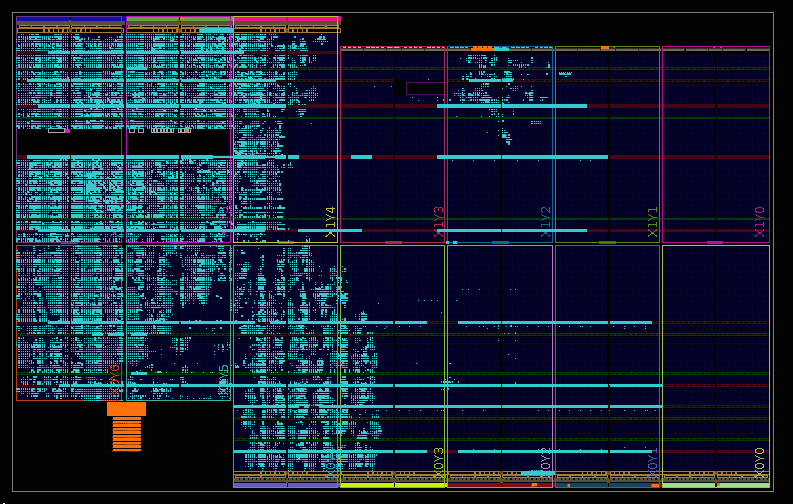
\includegraphics[width=\linewidth]{img/floorplan.png}
\end{minipage}
\begin{minipage}{0.45\linewidth}
\centering
\alert{Utilization} \\[0.5\baselineskip]
\footnotesize
\begin{tabular}{ | c | c | c |  } \hline
    Resource        & w/o A+TM & w/A+TM  \\ \hline
    Slice LUTs      & 17.09\%   &  21.79\%   \\  \hline
    Slice Registers & 6.18\%    &  8.01\%    \\  \hline
    Memory          & 21.65\%   &  63.85\%   \\  \hline
\end{tabular}
\end{minipage}

\end{block}

    \vspace{1ex}
    Our preliminary evaluation demonstrates that this approach shows a lot of
promise. However, investigation into better replacement policies will
likely yield improvements in system performance.

\subsection{Methodology}

In our experimental setup, we generated key-value pairs, placed them in
memcached, and performed a GET request for each key. We then measured the
latencies for a series of GET requests generated from a predetermined
probability distribution. These distributions include one checking only a
single key, a uniform distribution, a normal distribution, a Pareto
distribution, and a distribution based on the ETC workload from the Facebook
study \cite{AXFJP2012}.

\subsection{Results}

In our first benchmark, we compared the latency of our accelerator to the
latency of software memcached in responding to requests for a single key.
For this experiment, we set a single key on the accelerator and in the
unmodified memcached software. We then issued repeated GET requests with
small random delays in between and recorded the latency of each request.

\begin{figure}[t]
\begin{center}
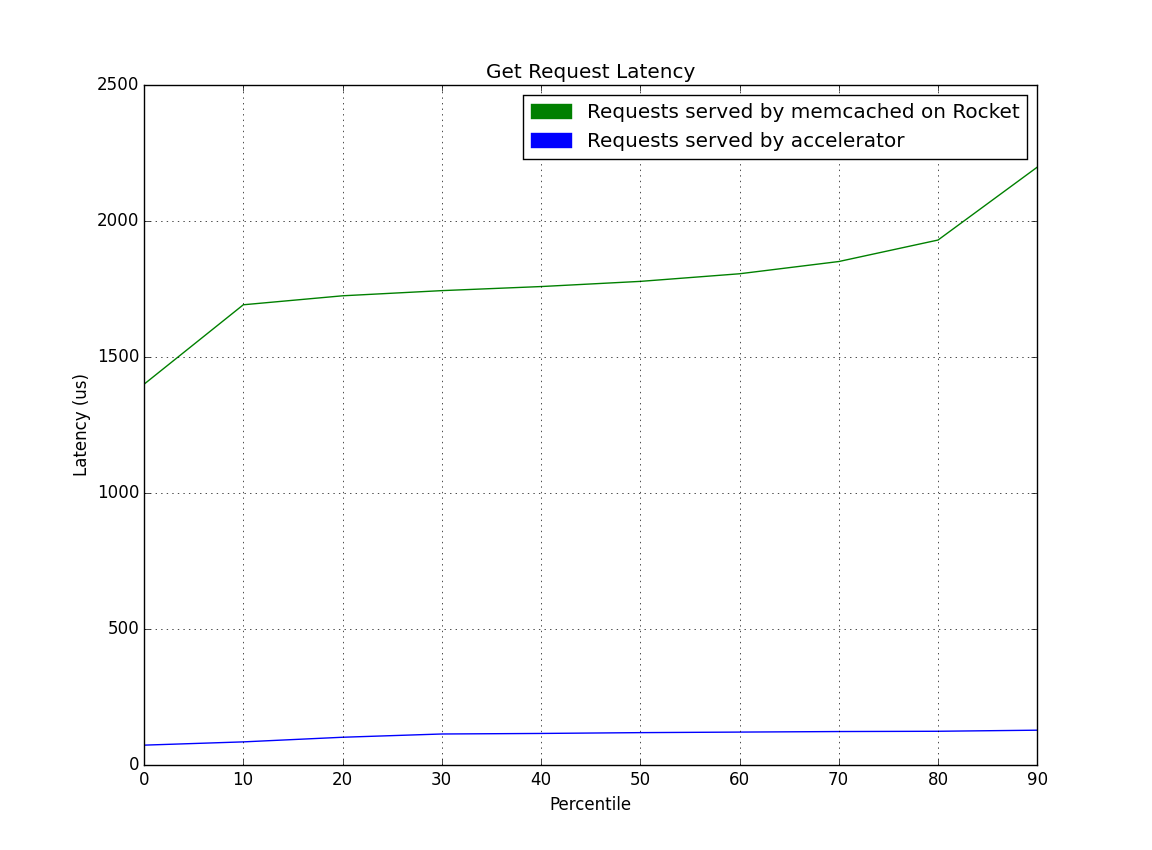
\includegraphics[width=\linewidth]{graph.png}
\caption{Latency of GET requests when only getting 1 key}
\label{fig:one-req}
\end{center}
\end{figure}

\begin{figure}[t]
\begin{center}
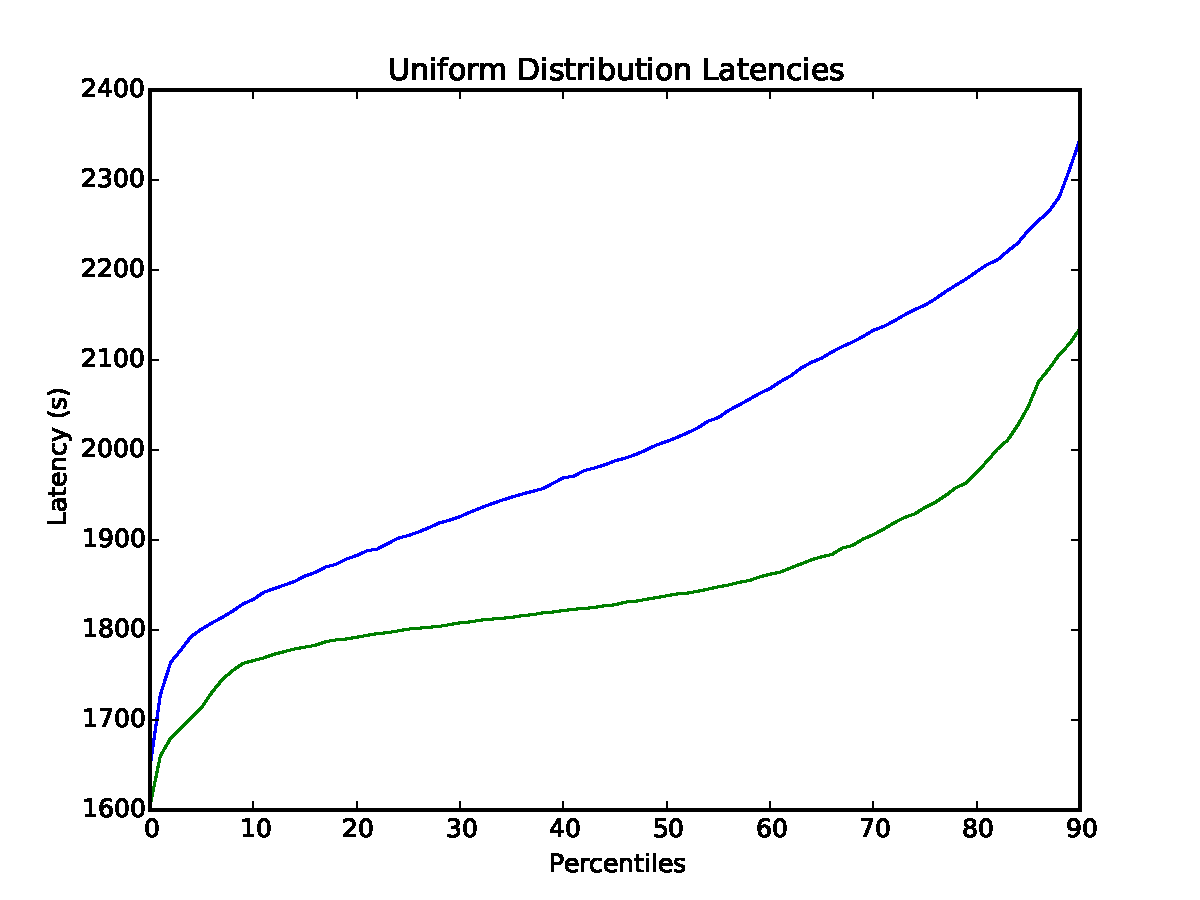
\includegraphics[width=\linewidth]{unif.pdf}
\caption{Latency of GET requests when keys follow a uniform distribution}
\label{fig:unif}
\end{center}
\end{figure}

\begin{figure}[t]
\begin{center}
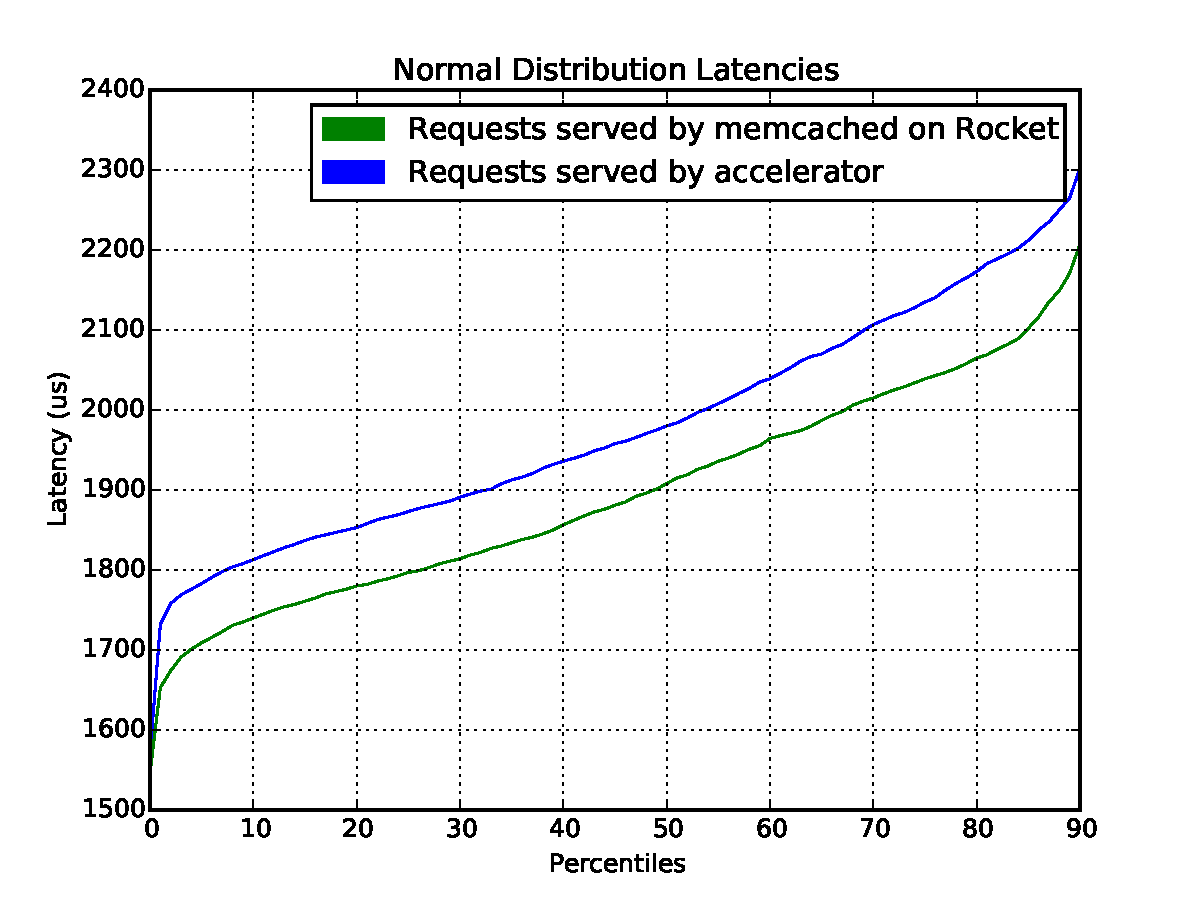
\includegraphics[width=\linewidth]{norm.pdf}
\caption{Latency of GET requests when keys follow a normal distribution}
\label{fig:norm}
\end{center}
\end{figure}

As we see from Figure \ref{fig:one-req}, there is approximately an order of
magnitude improvement between a request served by the accelerator and a
request served by memcached software running on the CPU.

After the single-key benchmark, we tested a series of requests chosen
according to a uniform distribution of keys.

In Figure \ref{fig:unif}, we see that, for this distribution, the
hardware-accelerated implementation performs worse than than the pure software
implementation. The driving factor behind the poor performance is the overhead
incurred in the traffic manager checking if each key is in the accelerator.
Since all requests on the accelerated implementation must pay this penalty,
we expect the accelerated implementation to perform poorly for key
distributions that are not heavily skewed. The results for a normal distribution
(Figure \ref{fig:norm}) show similarly poor performance for the accelerator
compared to the software implementation.

\begin{figure}[t]
\begin{center}
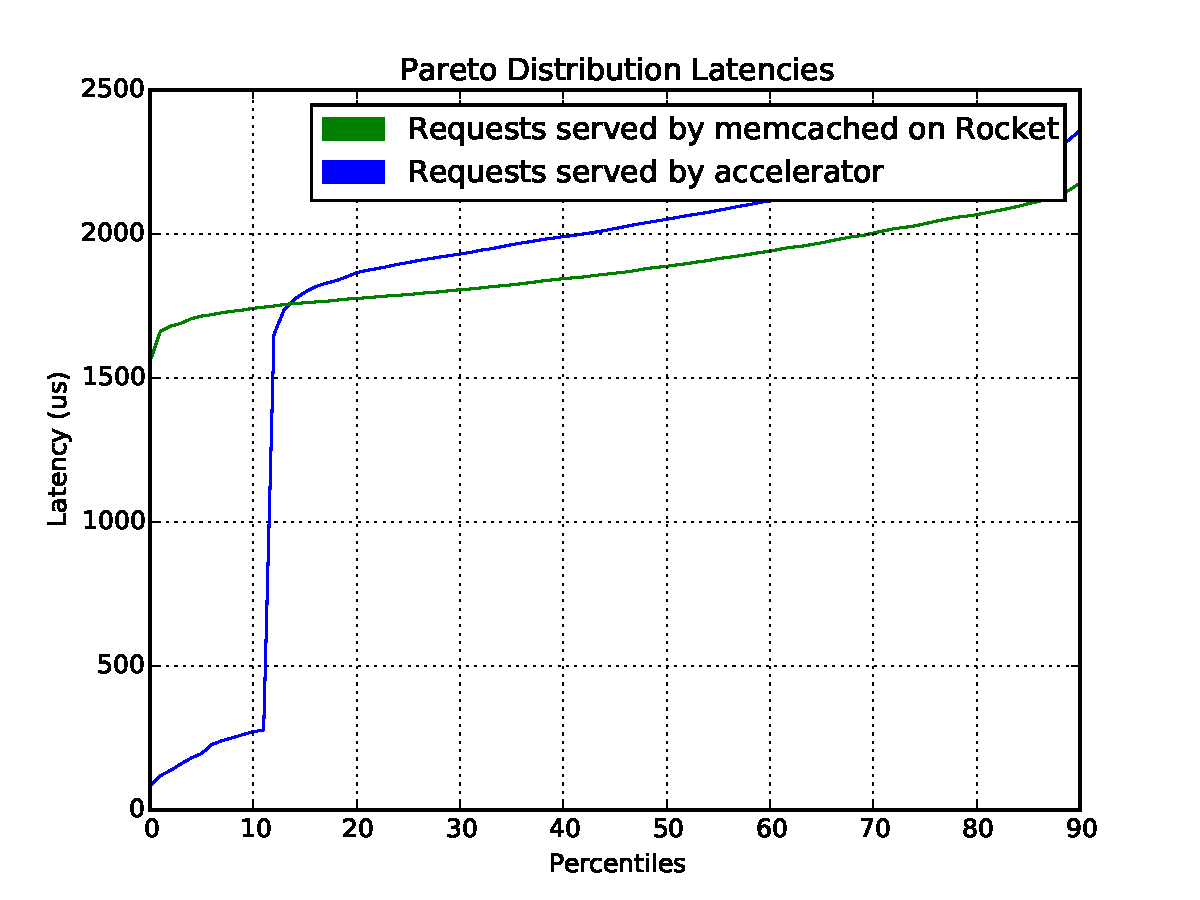
\includegraphics[width=\linewidth]{pareto.pdf}
\caption{Latency of GET requests when keys follow a pareto distribution}
\label{fig:pareto}
\end{center}
\end{figure}

\begin{figure}[t]
\begin{center}
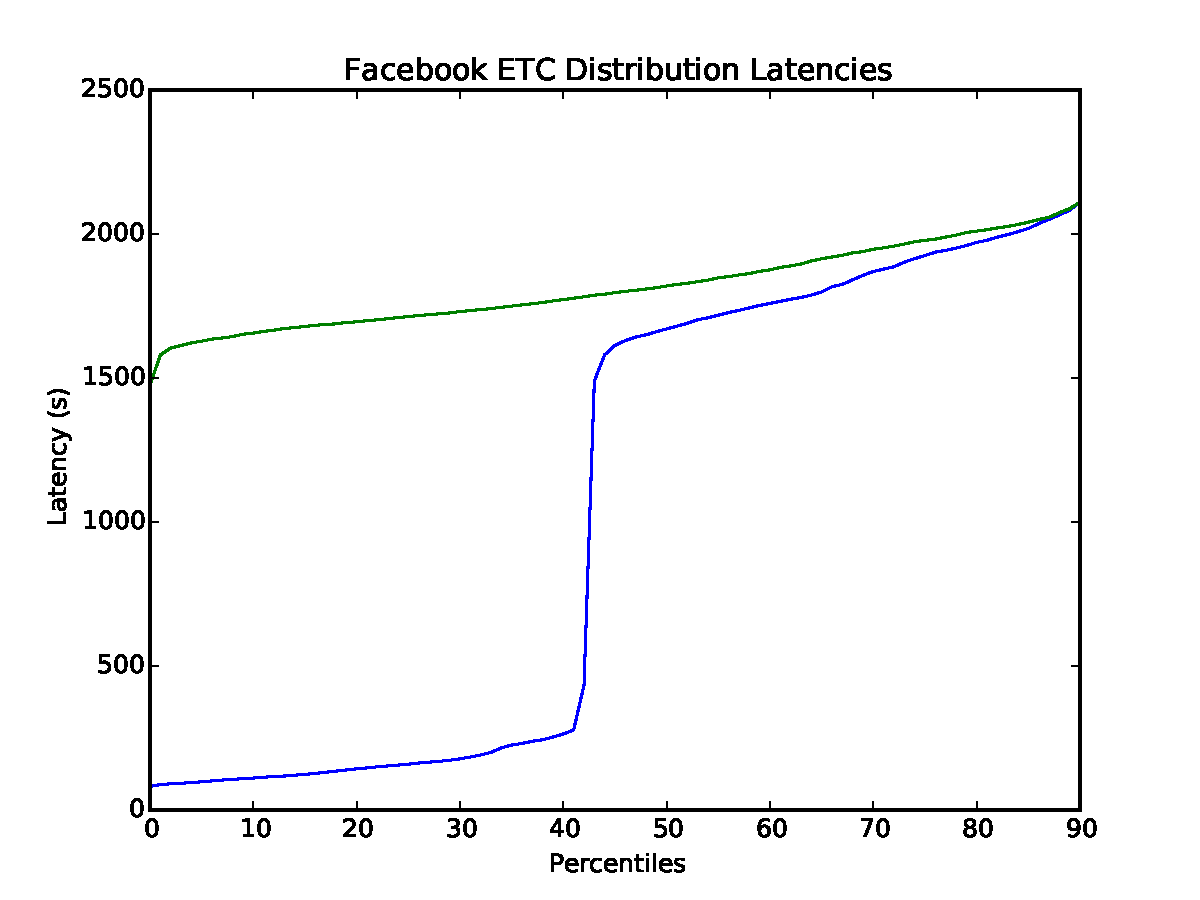
\includegraphics[width=\linewidth]{etc.pdf}
\caption{Latency of GET requests when keys follow the Facebook ETC distribution}
\label{fig:etc}
\end{center}
\end{figure}

For skewed distributions such as a Pareto distribution (Figure \ref{fig:pareto}),
we see a drastic improvement in the accelerated implementation over the
pure-software implementation. In this test, the most popular keys are placed
on the accelerator and are not easily evicted. For the these keys, the 10x
latency improvement from serving from the accelerator more than makes up
for the latency penalty incurred in the traffic manager. However, only about
$11\%$ of the requests benefit from acceleration. Requests for keys not placed
on the  accelerator still have higher latency than in the software implementation.

Finally, we used the Facebook ETC distribution \cite{AXFJP2012} in order to see
how our system would fare against a real-life workload. In Figure
\ref{fig:etc}, we see that this is a very promising start. $40$ percent of all
requests get a $10$ times improvement in latencies. However, the poor
performance in the non-skewed distributions suggests that improvements can be
made in our caching policy to enhance system performance.

    \vspace{1ex}
    \section{Conclusion}

In this paper, we described a hardware accelerator for the Memcached key-value
store which we developed and evaluated on the ZC706 FPGA development board.
By storing keys and values in a dedicated SRAM cache and serving responses
directly to the NIC without involving the CPU, our accelerator delivers an
order of magnitude improvement in latency. We furthermore showed that our
accelerator can store a number of key-value pairs sufficient to serve 40\% of
the requests in a real-world workload.

	\end{column}
\end{columns}
\end{frame}
\end{document}
